%-----------------------------------------
\begin{frame}
\frametitle{Motivating applications}
\begin{minipage}{0.45\textwidth}
    \begin{figure}      
    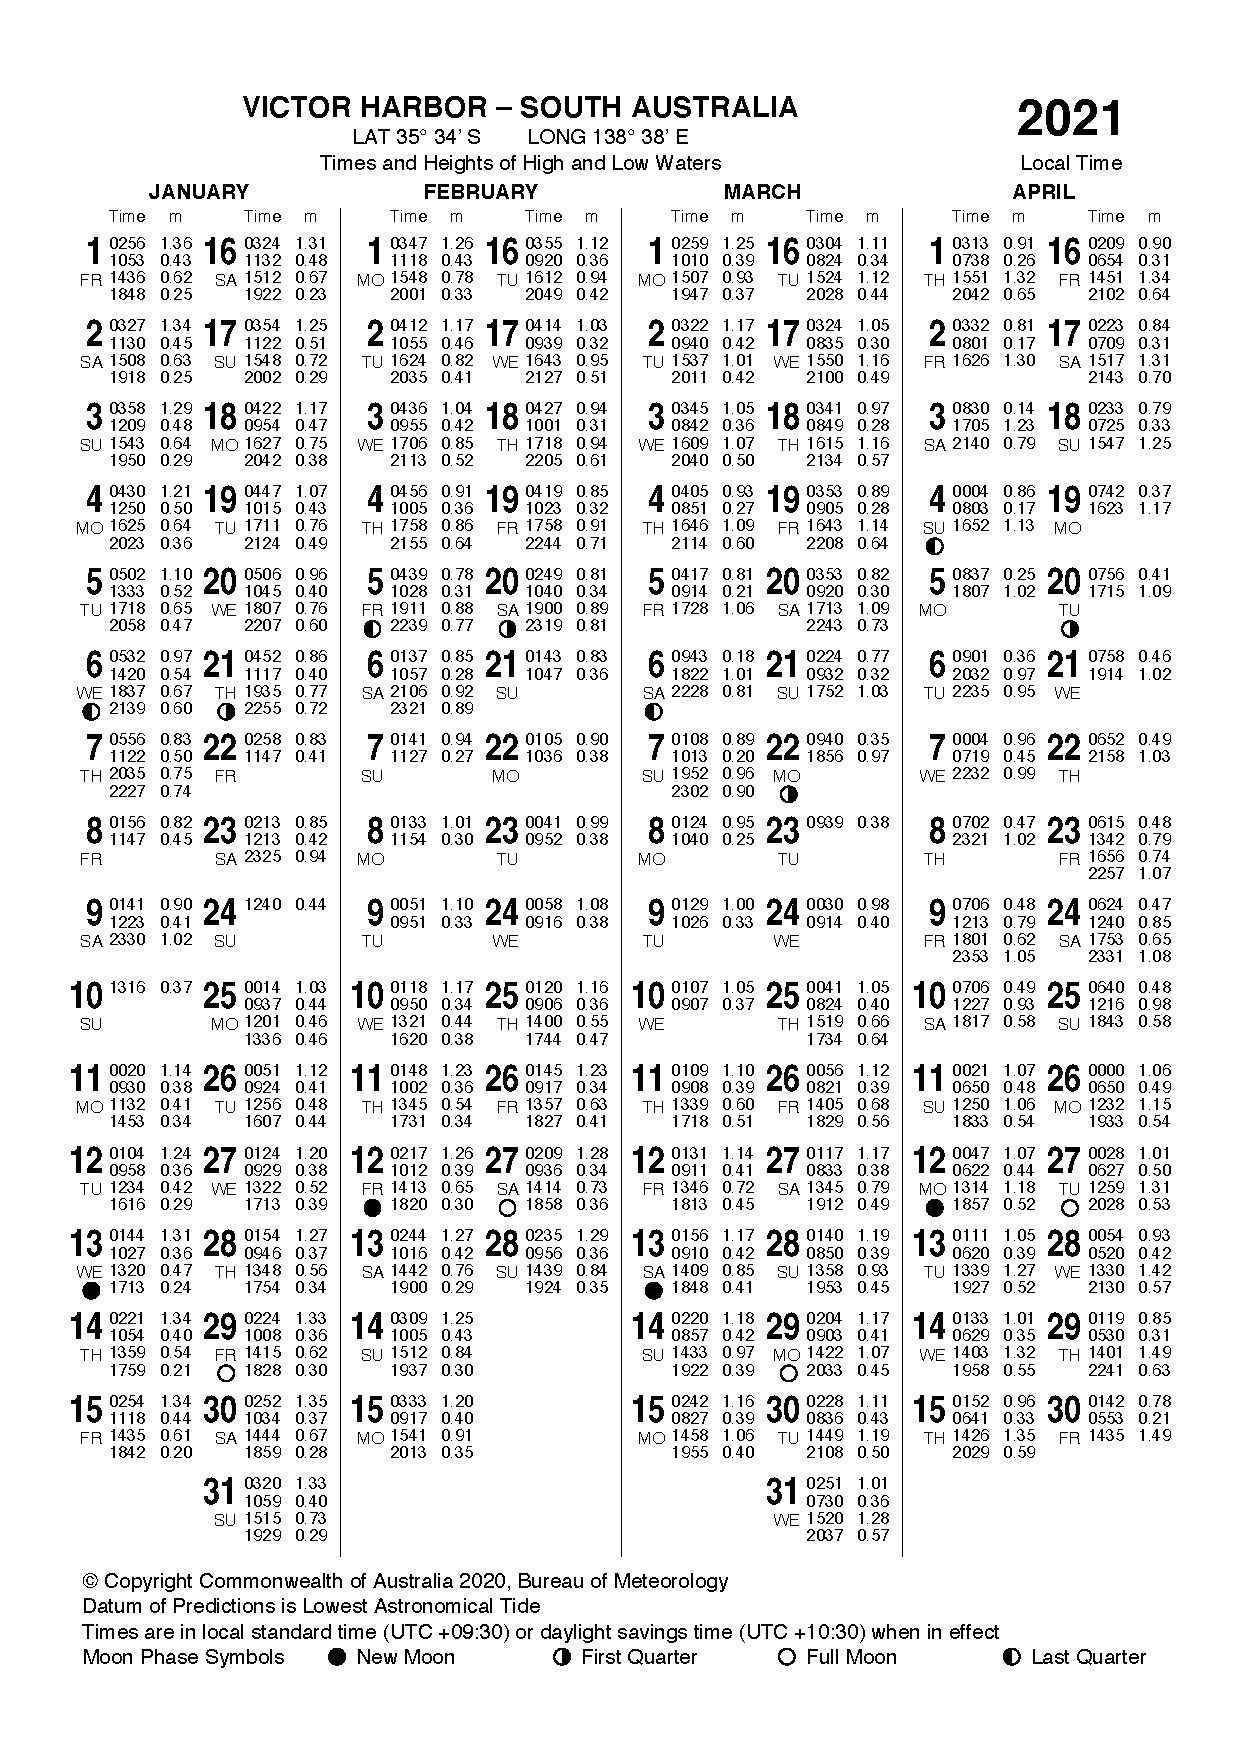
\includegraphics[width=\textwidth]{figures/images/IDO59001_2021_SA_TP006.pdf}
    \end{figure}
\end{minipage}
\hfill
\begin{minipage}{0.45\textwidth}
    \begin{figure}      
     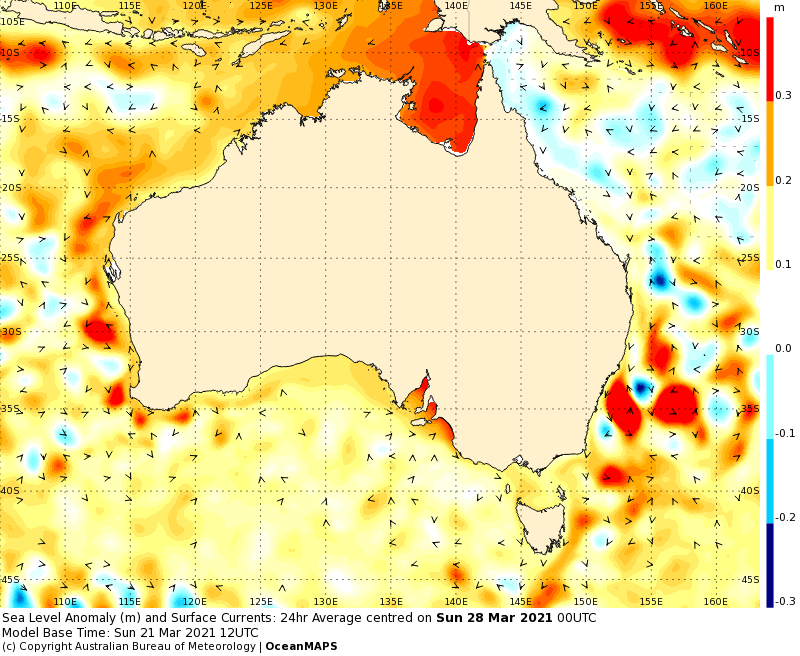
\includegraphics[width=\textwidth]{figures/images/IDYOC300.Aus.SLACur.168.png}
    \end{figure} 
\end{minipage}
\end{frame}
%-----------------------------------------
\begin{frame}
\frametitle{Motivating applications}
\begin{minipage}{0.45\textwidth}
    \begin{figure}      
    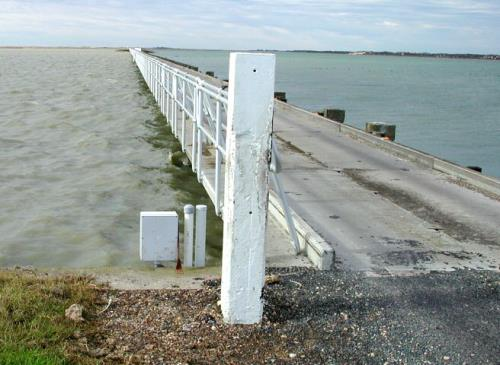
\includegraphics[width=\textwidth]{figures/images/goolwa_ewe_island-environment_sa_gov_au.jpg}
    \end{figure}
\end{minipage}
\hfill
\begin{minipage}{0.45\textwidth}
    \begin{figure}      
     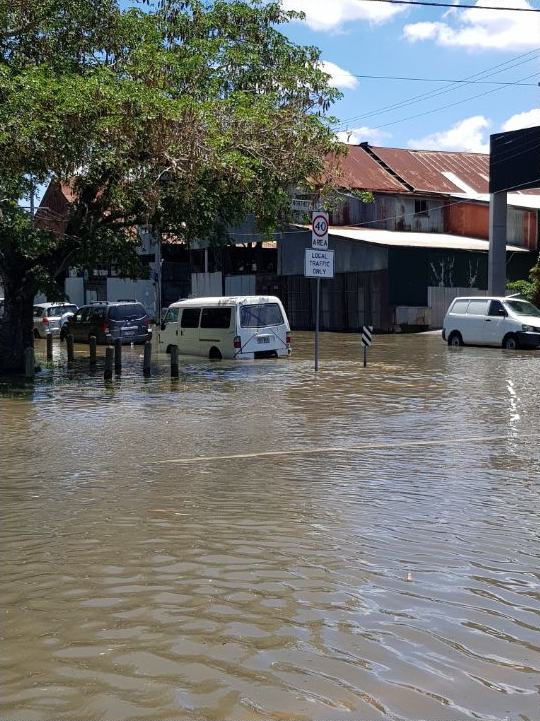
\includegraphics[width=\textwidth]{figures/images/sunnyFlood_ClarkJan2018Brisbane.png}
    \end{figure} 
\end{minipage}

\end{frame}
%-----------------------------------------
\begin{frame}
\frametitle{Motivating applications}
\begin{minipage}{0.45\textwidth}
    \begin{figure}      
    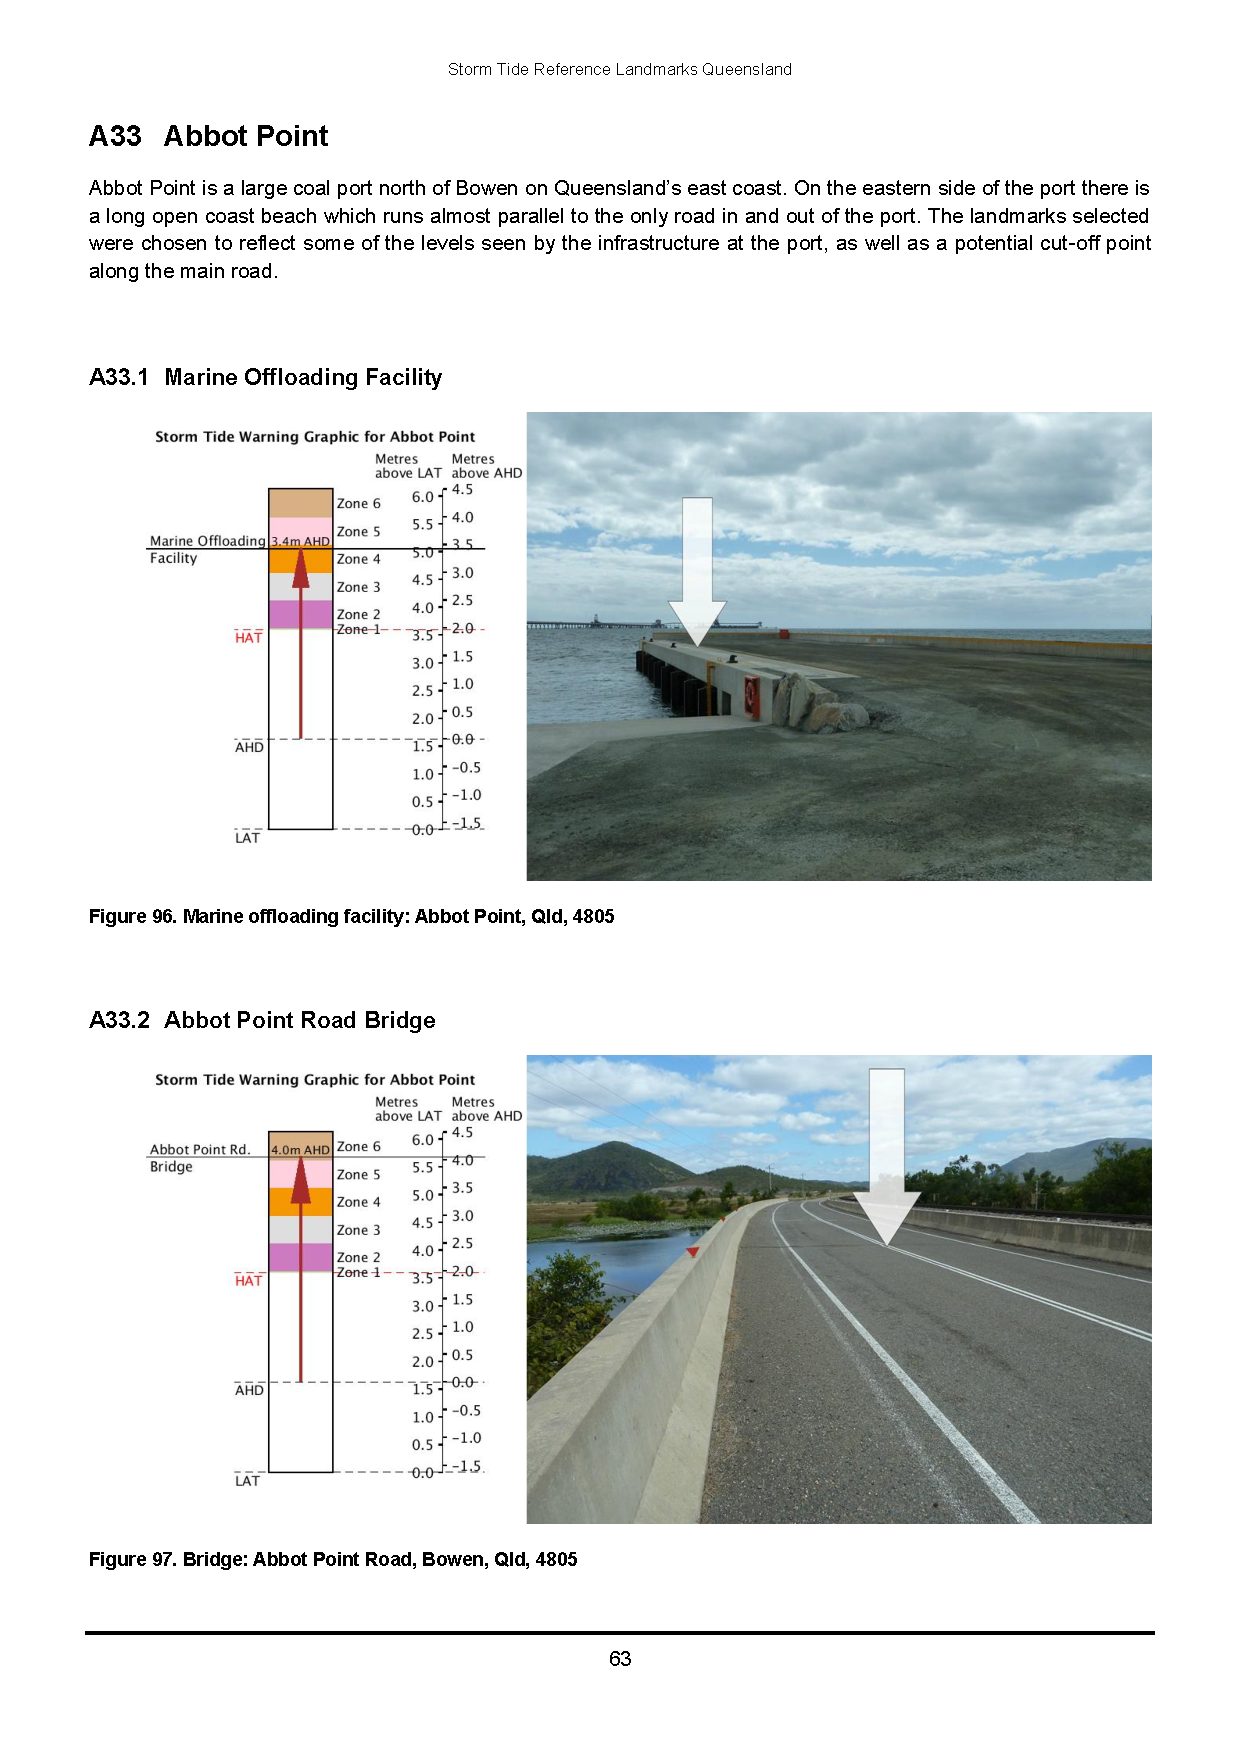
\includegraphics[width=\textwidth]{figures/images/qldLandmarkEg.pdf}
    \end{figure}
\end{minipage}
\hfill
\begin{minipage}{0.45\textwidth}
  Text
\end{minipage}

\end{frame}
% - MW/Goolwa/weirs, Nuisance or sunny, 
% - in homogeneous guidance: what to do with it?
% SLA map, tide table, surge tide > HAT, seasonal, river forecast tide 
